{\color{indiagreen}\subsection{Enakomerno gibanje}}
To je gibanje pri katerem je \textbf{hitrost konstantna}. Primer: krogla, ki jo iztrelimo v breztežnostnem prostoru.\\
\begin{align*}
	a &=0\\
	v &= v_0\\
	s &= v_0 * t \rightarrow v_0 = \frac{s}{t}\\
	v^2 &= v_0^2\\
\end{align*}

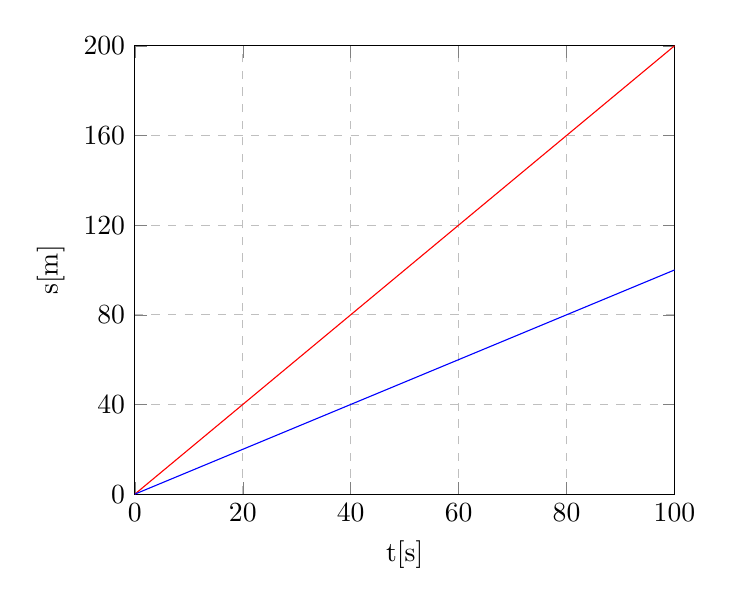
\begin{tikzpicture}
\begin{axis}[
    xlabel={t[s]},
    ylabel={s[m]},
    xmin=0, xmax=100,
    ymin=0, ymax=200,
    xtick={0,20,40,60,80,100},
    ytick={0,40,80,120,160,200},
    ymajorgrids=true,
    xmajorgrids=true,
    grid style=dashed,
]
 
\addplot[
    color=red,
    ]
    coordinates {

    (0,0)(100,200)
    };
\addplot[
    color=blue,
    ]
    coordinates {

    (0,0)(100,100)
    };
 
\end{axis}
\end{tikzpicture}

Naklon pove hitrost\\
\begin{align*}
	f &= tan \alpha = k\\
	k &= \frac{\Delta y}{\Delta x} = \frac{\Delta s}{\Delta t} = v\\
\end{align*}

\begin{tikzpicture}
\begin{axis}[
    xlabel={t[s]},
    ylabel={v[m]},
    xmin=0, xmax=100,
    ymin=0, ymax=200,
    xtick={0,20,40,60,80,100},
    ytick={0,40,80,120,160,200},
    ymajorgrids=true,
    xmajorgrids=true,
    grid style=dashed,
]
 

\addplot[
    color=red,
    ]
    coordinates {

    (0,150)(100,150)
    };
\addplot[
	name path=odkje,
    color=blue,
    ]
    coordinates {

    (0,100)(100,100)
    };
    \path[name path=dokam] (axis cs:0,0) -- (axis cs:100,0);

    \addplot [
        thick,
        color=blue,
        fill=blue, 
        fill opacity=0.5
    ]
    fill between[
        of=odkje and dokam,
        soft clip={domain=0:100},
    ];
 
\end{axis}
\end{tikzpicture}

\textbf{Ploščina} pod krivuljo nam pove prepotovano pot.\\
\begin{align*}
	s &= t * v\\
\end{align*}